\documentclass[11pt,a4paper]{article}
\usepackage[utf8]{inputenc}
\usepackage[T1]{fontenc}
\usepackage[english]{babel}
\usepackage[top=2.5cm,bottom=2.2cm,left=2.2cm,right=2.2cm,headheight=25pt,headsep=16pt]{geometry}
\usepackage{graphicx,xcolor,booktabs,tabularx,array,float,tikz,enumitem,listings,fancyhdr,hyperref,caption,titlesec}
\usetikzlibrary{arrows.meta,positioning,shapes.geometric}
\newcolumntype{Y}{>{\raggedright\arraybackslash}X}
\hypersetup{colorlinks=true,linkcolor=blue,urlcolor=blue,hypertexnames=false}
\setlength{\parskip}{4pt}\setlength{\parindent}{0pt}\renewcommand{\arraystretch}{1.18}
\setlist{nosep,leftmargin=*}
\definecolor{primary}{RGB}{20,60,120}\definecolor{accent}{RGB}{0,120,180}\definecolor{navy}{HTML}{17365D}\definecolor{teal}{HTML}{168C9A}\definecolor{pale}{HTML}{EFF5F8}
\graphicspath{{figures/}{../solution1/resolucion-actividad1/evidencias/}{evidencias/}}
\pagestyle{fancy}\fancyhf{}
\fancyhead[L]{\small\color{primary}\textbf{Distributed Systems} \textbar\ Workshop 6}
\fancyhead[R]{\small\color{primary}Yachay Tech University}
\fancyfoot[C]{\small\thepage}
\renewcommand{\headrulewidth}{0.5pt}
\renewcommand{\headrule}{\hbox to\headwidth{\color{primary!50}\leaders\hrule height \headrulewidth\hfill}}
\titleformat{\section}{\Large\bfseries\color{primary}}{\thesection.}{0.6em}{}[\vspace{2pt}{\color{primary!40}\titlerule[0.8pt]}\vspace{4pt}]
\titleformat{\subsection}{\bfseries\color{primary!80}}{\thesubsection}{0.5em}{}
\lstset{basicstyle=\ttfamily\small,backgroundcolor=\color{pale},frame=single,breaklines=true}
\begin{document}
\begin{titlepage}\thispagestyle{empty}\centering
\noindent\begin{minipage}[t]{0.48\textwidth}\small\color{primary}\textbf{Distributed Systems} \textbar\ Workshop 6\end{minipage}\hfill\begin{minipage}[t]{0.48\textwidth}\raggedleft\small\color{primary}Yachay Tech University\end{minipage}\\[-2pt]
{\color{primary}\rule{\textwidth}{0.5pt}}\\[1.15cm]
\noindent\begin{minipage}[c]{0.23\textwidth}\raggedright
\includegraphics[width=3.4cm,height=1.2cm,keepaspectratio]{logo1.png}\end{minipage}\hfill
\begin{minipage}[c]{0.48\textwidth}\centering{\large\bfseries\color{primary}Yachay Tech University}\\[-1pt]{\small School of Mathematical and Computational Sciences}\\[3pt]{\small\color{primary}Course: Distributed Systems | Workshop 6}\end{minipage}\hfill
\begin{minipage}[c]{0.23\textwidth}\raggedleft
\includegraphics[width=4.0cm,height=1.2cm,keepaspectratio]{logo2.png}\end{minipage}\\[0.75cm]
{\color{primary}\rule{\textwidth}{1.2pt}}\\[0.9cm]{\Huge\bfseries Workshop 6}\\[0.35cm]
{\LARGE Distributed Middleware with RabbitMQ}\\[0.5cm]
{\large Activity 1: C/Python Comparison}\\
{\large Activity 2: Federated Learning Architecture}\\[0.6cm]
{\color{primary}\rule{\textwidth}{1.2pt}}\\[1.4cm]
{\large\textbf{Student:} Dario Pomasqui}\\[0.25cm]
{\large\textbf{Course:} Distributed Systems -- Semester II 2026}\\[0.25cm]
{\large\textbf{Instructor:} Prof. Francisco Hidrobo}\\[0.25cm]
{\large October 22, 2026}\\[0.2cm]{\small\href{https://github.com/adrianasofiaespinoza/Sistemas-Distribuidos/tree/main/Workshop6}{Workshop 6 project repository on GitHub}}\\[1cm]
\vfill\end{titlepage}\section*{Abstract}This report documents both Workshop 6 activities. Activity 1 runs the RabbitMQ point-to-point queue and fanout examples in Python, then installs \texttt{librabbitmq-dev} in a reproducible Ubuntu environment to build and run the C producer and consumer. Activity 2 designs and implements a RabbitMQ communication prototype for the federated learning project on leaf disease detection. Three farm processes exchange instructions and updates; the coordinator computes FedAvg with all clients and with a partial quorum. Tests validate message transport, acknowledgments, and aggregation using synthetic values. They do not train a CNN or measure classification accuracy.
\section{Context and Objectives}The project proposal compares FedAvg and FedProx for leaf disease classification using non-IID data distributed across Farm A, Farm B, and Farm C. Each farm keeps its images locally and performs local training. A coordinator receives parameter updates, aggregates them according to sample counts, and manages training rounds.

The initial proposal described RPC with Flower without specifying queues, delivery confirmations, or failure recovery. For this submission, the architecture uses RabbitMQ over AMQP 0-9-1 and the Pika Python client. The project proposal source at \texttt{../../proporsal/proposal.tex} was updated with this design and distinguishes model synchronization from distributed consensus.
\section{Activity 1: RabbitMQ and Client Comparison}
\subsection{What the Activity 1 Folder Contains}
I organized the supplied examples by communication pattern and implementation language. The \texttt{python-basic/} folder contains \texttt{producer.py}, \texttt{consumer.py}, and their Pika dependency list; these files demonstrate point-to-point messaging through the \texttt{hello} queue. The \texttt{python-pubsub/} folder contains \texttt{pub.py}, \texttt{sub.py}, and its requirements file; these demonstrate fanout publication to multiple subscribers. The \texttt{c-basic/} folder contains the C producer, consumer, and Makefile used to build the AMQP clients.

I added \texttt{../solution1/resolucion-actividad1/} to document and reproduce my work. It contains this activity's Markdown report, the PowerShell test script, a Dockerfile for the C build environment, and \texttt{evidencias/} with broker screenshots, command output, and inspection notes. The original examples remain in their respective folders; the added folder records how I tested them and what I observed.

\subsection{Environment and Procedure}
\begin{itemize}\item I started the \texttt{rabbitmq:3-management} Docker image as my broker (RabbitMQ 3.13.7). I used AMQP port 5672 for clients and port 15672 for the Management UI.\item I used Python 3.13.14 with Pika 1.4.4 and ran the four supplied Python programs: the queue producer and consumer, and the fanout publisher and subscriber.\item To compile the C examples, I built the Docker image \texttt{workshop6-c-dev} on Ubuntu 24.04 with \texttt{build-essential} and \texttt{librabbitmq-dev} 0.11.0-1ubuntu0.2. I then used the supplied Makefile to build both programs.\item I also updated the C examples to accept an optional \texttt{RABBITMQ\_HOST} value and to check connection, channel, and publish errors.\end{itemize}
I recorded the repeatable steps in \texttt{../solution1/resolucion-actividad1/ejecutar-pruebas.ps1}. I can run the script from that folder after starting the broker; it requires Docker Desktop and Python:\begin{lstlisting}
powershell.exe -NoProfile -ExecutionPolicy Bypass -File .\ejecutar-pruebas.ps1
\end{lstlisting}
\subsection{Tests and Results}\begin{table}[H]\small\centering\begin{tabularx}{\textwidth}{p{3.1cm}p{1.5cm}Y}\toprule
Test & Result & Observation \\\midrule
Pika AMQP connection & PASS & Connected to \texttt{localhost:5672}. \\
Python queue & PASS & \texttt{Hello Middleware!} published, received, and acknowledged; durable queue \texttt{hello}, QoS 1. \\
Python fanout & PASS & Both exclusive queues received \texttt{Workshop6 fanout test}. \\
Python syntax & PASS & All four scripts passed \texttt{py\_compile}. \\
C compilation & PASS & \texttt{make} built producer and consumer, linking \texttt{-lrabbitmq}. \\
C queue & PASS & Consumer received \texttt{Hello from C!} and sent an ack. \\
\bottomrule\end{tabularx}\caption{Activity 1 functional tests.}\end{table}
\begin{figure}[H]\centering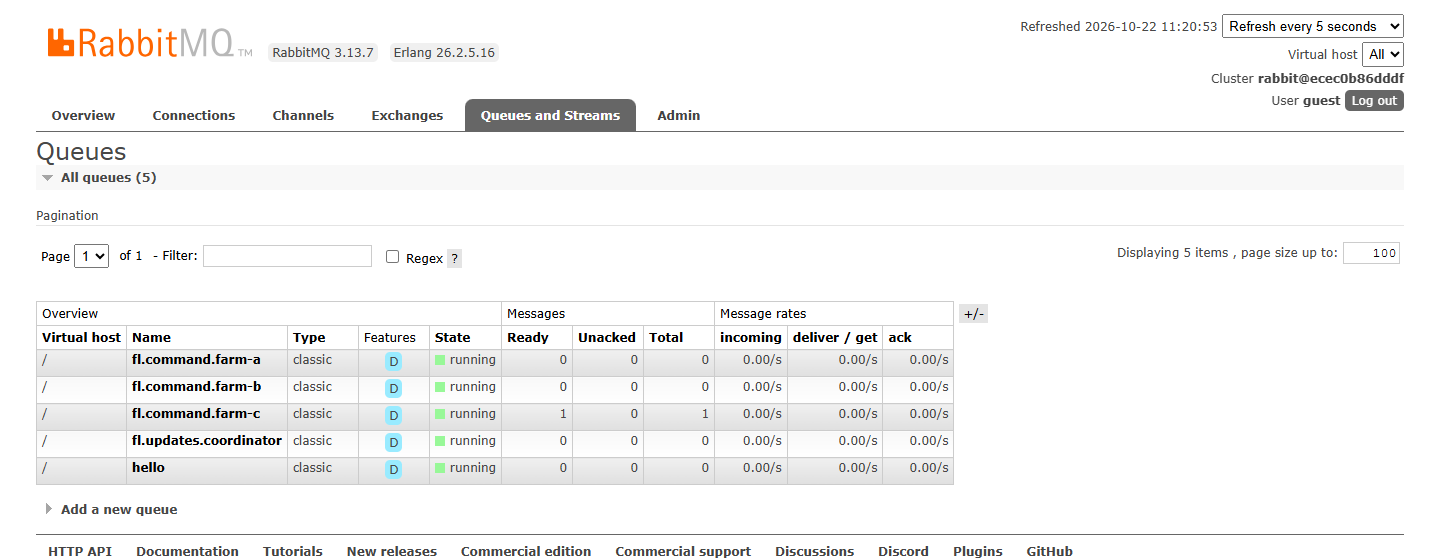
\includegraphics[width=.91\textwidth]{rabbitmq-cola-hello-crop.png}\caption{RabbitMQ Management: durable \texttt{hello} queue with no pending messages after the test.}\end{figure}
\begin{figure}[H]\centering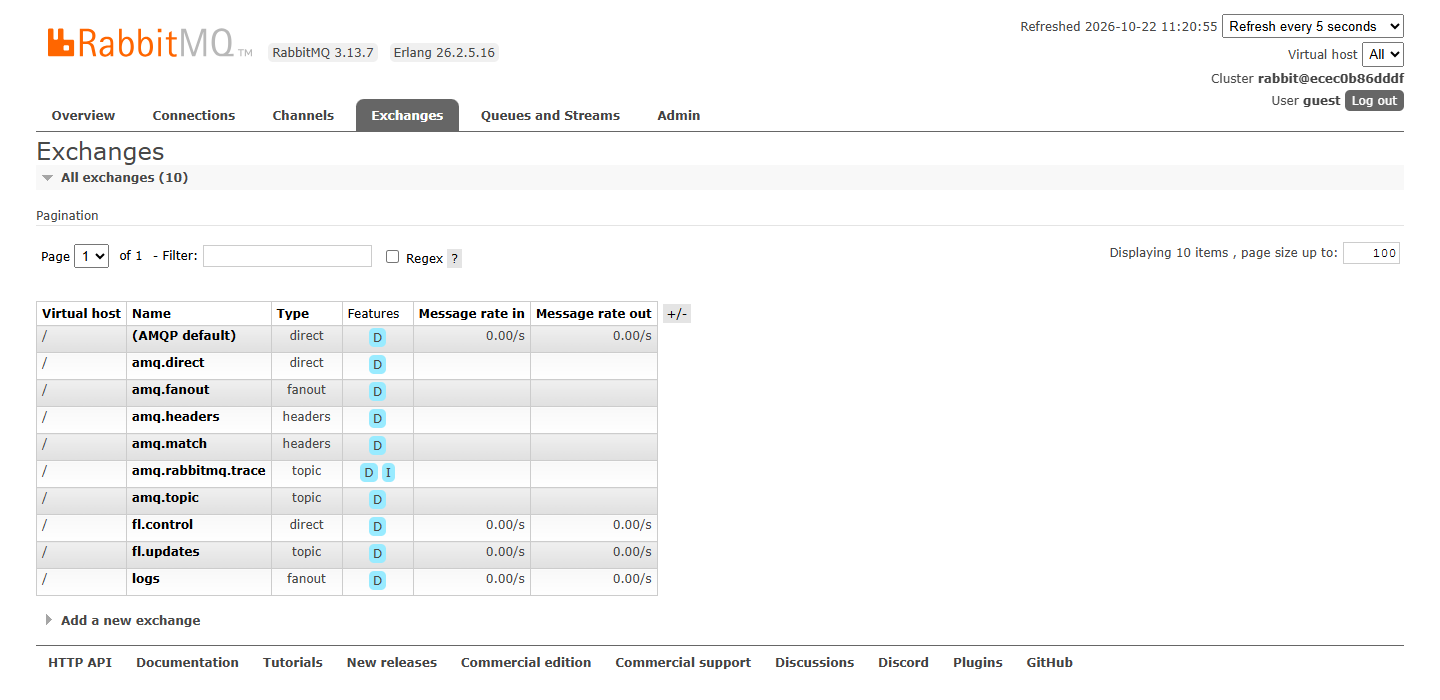
\includegraphics[width=.91\textwidth]{rabbitmq-exchange-logs-crop.png}\caption{Observed exchanges: example \texttt{logs} fanout exchange and Activity 2 exchanges.}\end{figure}
\subsection{C and Python Comparison}\begin{table}[H]\small\centering\begin{tabularx}{\textwidth}{p{2.4cm}YY}\toprule
Aspect & Python (Pika) & C (rabbitmq-c) \\\midrule
Interface & High-level API and callbacks; few lines are needed to publish and consume. & Explicit control of sockets, connections, channels, bytes, and message envelopes. \\
Dependencies & Python interpreter and Pika package. & Compiler, Make, headers, and library; installed here in Ubuntu Docker. \\
Delivery & Durable queue, persistent message, QoS 1, and manual acknowledgment. & Durable queue, persistent message, and manual acknowledgment. \\
Suitability & Straightforward integration with PyTorch and Python code. & Suitable for native components or existing C systems. \\
\bottomrule\end{tabularx}\caption{Implementation comparison.}\end{table}
By running both clients against the same AMQP broker, I confirmed that the language does not change the queue behavior. For this machine learning project, I find Python easier to integrate with the model code. C gives me more low-level control, but I need to manage its compiler and native library dependencies.
\section{Activity 2: Middleware for the Project}\subsection{Architecture}The topology is hub-and-spoke with a \textbf{single logical writer} for the global model. RabbitMQ routes and stores messages; the coordinator keeps round state and computes aggregations. Each farm is an independent process with private images and a local model copy.
\begin{figure}[H]\centering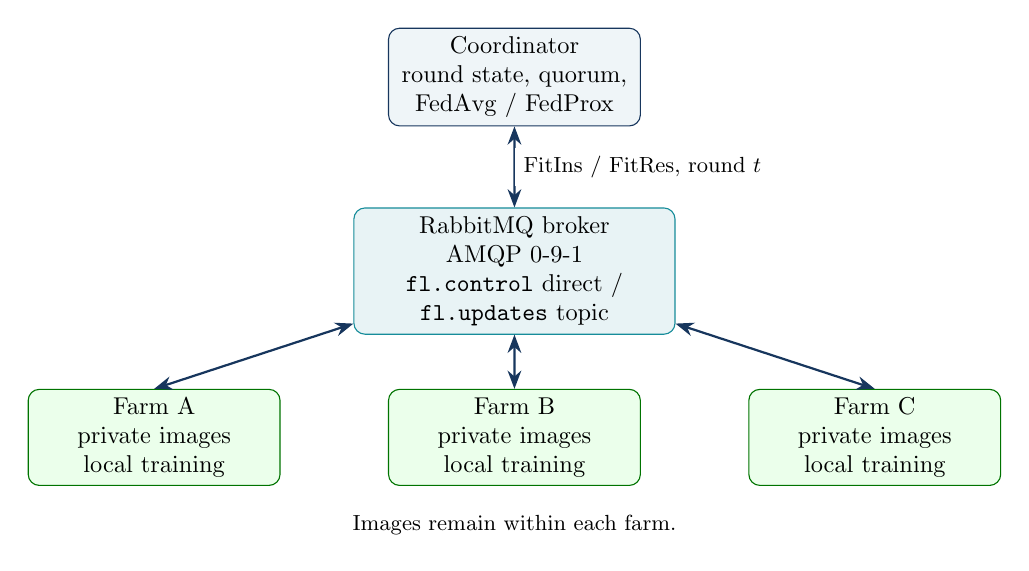
\begin{tikzpicture}[scale=.88,transform shape,box/.style={draw=navy,fill=pale,rounded corners,align=center,minimum height=1cm,text width=3.4cm},farm/.style={box,fill=green!8,draw=green!45!black},broker/.style={box,fill=teal!10,draw=teal,text width=4.4cm},arr/.style={{Stealth}-{Stealth},thick,draw=navy}]
\node[box] (coord) at (0,0) {Coordinator\\round state, quorum,\\FedAvg / FedProx};\node[broker] (broker) at (0,-2.8) {RabbitMQ broker\\AMQP 0-9-1\\\texttt{fl.control} direct / \texttt{fl.updates} topic};
\node[farm] (a) at (-5.2,-5.2) {Farm A\\private images\\local training};\node[farm] (b) at (0,-5.2) {Farm B\\private images\\local training};\node[farm] (c) at (5.2,-5.2) {Farm C\\private images\\local training};
\draw[arr] (coord) -- node[right,font=\small,fill=white]{FitIns / FitRes, round $t$} (broker);\draw[arr] (broker) -- (a.north);\draw[arr] (broker) -- (b.north);\draw[arr] (broker) -- (c.north);\node[draw=none,fill=none,below=.3cm of b,font=\small]{Images remain within each farm.};\end{tikzpicture}
\caption{Architecture tested with local processes. Instructions and results flow through the broker; deployment will connect remote nodes using TLS.}\end{figure}
\subsection{Exchanges, Queues, and Messages}\begin{table}[H]\small\centering\begin{tabularx}{\textwidth}{p{3cm}p{4cm}Y}\toprule
Flow & RabbitMQ & Purpose \\\midrule
Coordinator $\to$ farm & Durable direct exchange \texttt{fl.control}; queue \texttt{fl.command.<farm-id>} per node & \texttt{FitIns}: round identifiers, global model, and configuration. \\
Farm $\to$ coordinator & Durable topic exchange \texttt{fl.updates}; queue \texttt{fl.updates.coordinator}, binding \texttt{fit.*.*} & \texttt{FitRes}: round, client, sample count, parameters, and metrics. \\
Future observability & Topic exchange \texttt{fl.events} & Completed rounds, timeouts, and failures. \\
\bottomrule\end{tabularx}\caption{AMQP routing.}\end{table}
Messages include \texttt{message\_id}, \texttt{correlation\_id=round\_id}, type, and schema version. Farms use manual acknowledgments and publisher confirms before acknowledging an instruction. The coordinator validates round and client identifiers, discards duplicates and stale results, and counts each client only once.
\subsection{Failures, Consistency, and Rationale}AMQP delivery can be repeated, so the application performs deduplication and does not claim exactly-once delivery. The coordinator completes a round when the configured quorum is reached or the deadline expires. Only then does it publish the next global version. If quorum is not reached, it retains the previous version. Disconnected clients keep instructions in durable queues and must install the current version when reconnecting.

FedAvg is not a consensus protocol such as Raft or Paxos. The coordinator is a single logical writer; tolerating its failure requires durable checkpoints and leader election or fencing. Replicating only the broker does not prevent two active coordinators. During a partition, local inference may continue, but a global model is not committed without the required update threshold.

RabbitMQ decouples local training time from coordinator availability, routes results by key, and stores work while a client is disconnected. A direct exchange routes instructions to each farm, while a topic exchange collects results. Pika and rabbitmq-c both support the protocol, enabling interoperability.

The broker alone does not provide differential privacy, secure aggregation, or Byzantine fault tolerance. Deployment requires TLS, per-node credentials and virtual hosts, resource limits, payload validation, and protection for model updates. CNN tensors should use an efficient binary format; JSON is used only in this prototype.
\subsection{Functional Tests}Processes exchanged synthetic scalar updates to validate transport and FedAvg averaging; the dataset was not loaded and PyTorch was not used for training.
\begin{table}[H]\small\centering\begin{tabularx}{\textwidth}{p{3cm}YY}\toprule
Test & Inputs & Result \\\midrule
Three farms & Initial weight 0; A: $n=10,w=1$; B: $n=20,w=2$; C: $n=30,w=4$. & A/B/C published and received acknowledgments. $w=(10+40+120)/60=2.8333$; \texttt{quorum\_complete}. \\
Farm C offline & A/B active; minimum quorum 2. & A/B contributed; C's instruction remained pending in its durable queue. $w=(10+40)/30=1.6667$; \texttt{partial\_quorum}. \\
Unit tests & Averaging, incompatible dimensions, and non-positive sample counts. & 3 of 3 passed. \\
\bottomrule\end{tabularx}\caption{Activity 2 tests.}\end{table}
\begin{figure}[H]\centering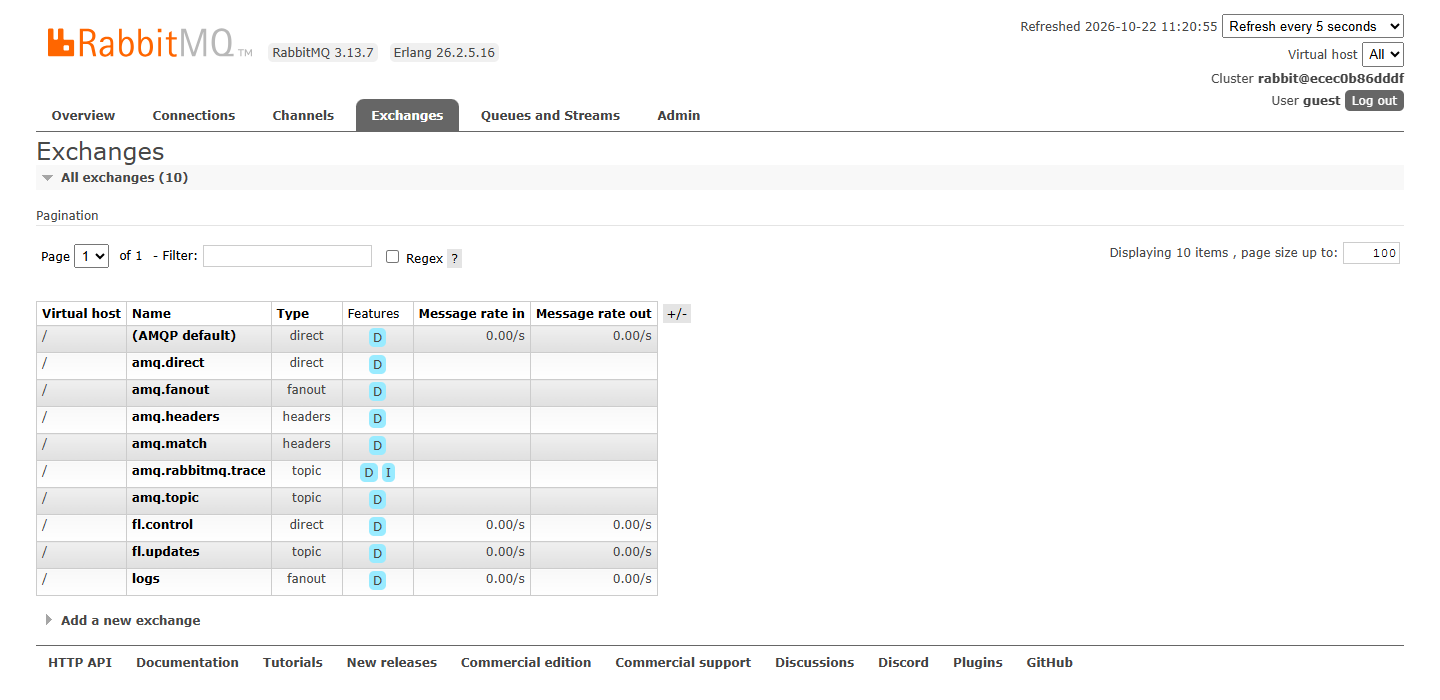
\includegraphics[width=.91\textwidth]{rabbitmq-exchanges-crop.png}\caption{Live exchanges: \texttt{fl.control} direct and \texttt{fl.updates} topic.}\end{figure}
\begin{figure}[H]\centering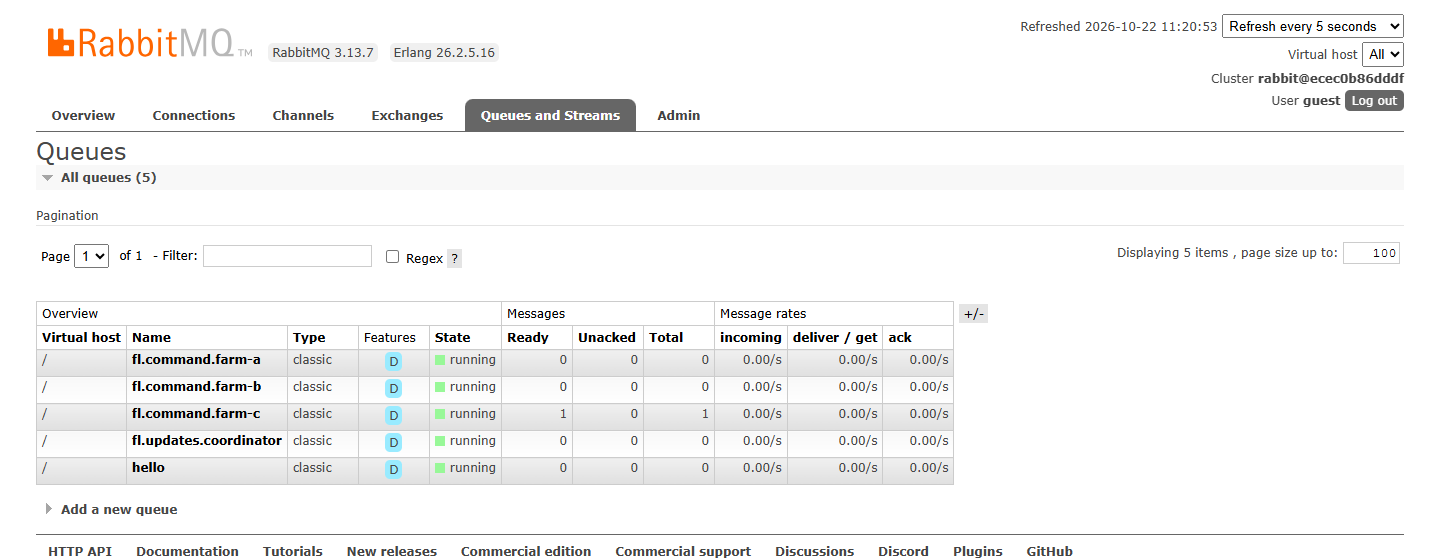
\includegraphics[width=.91\textwidth]{rabbitmq-queues-dropout-crop.png}\caption{Farm C offline: its durable instruction remains pending (Ready=1).}\end{figure}
\begin{figure}[H]\centering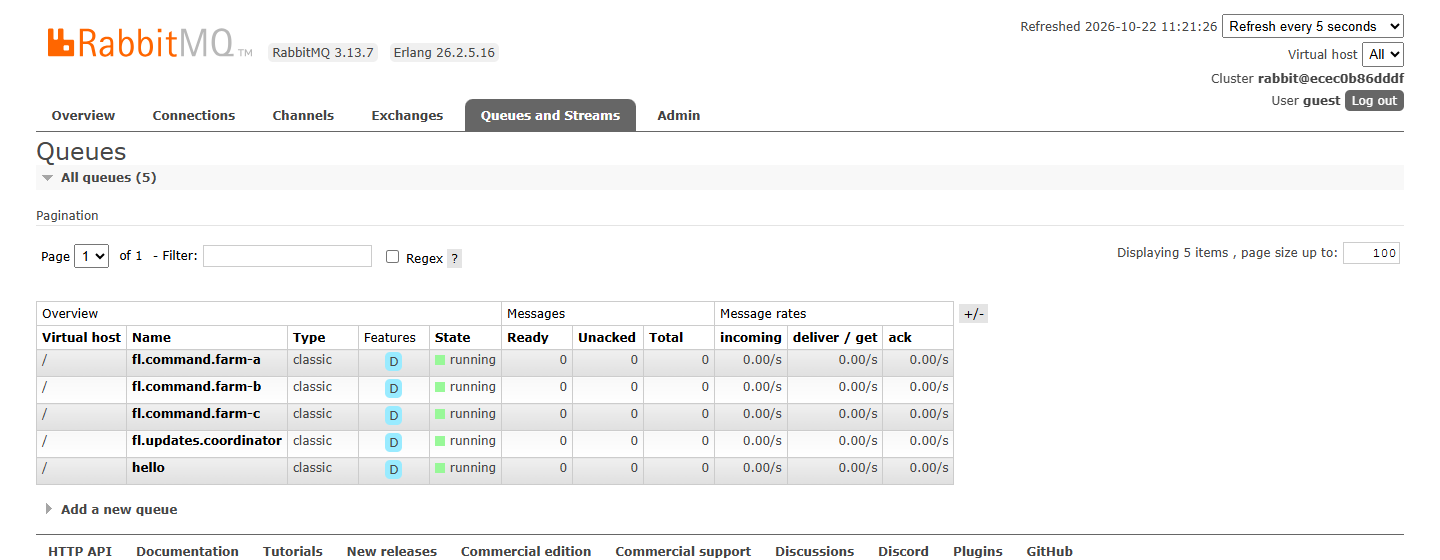
\includegraphics[width=.91\textwidth]{rabbitmq-queues-three-farms-crop.png}\caption{After the complete round, all five queues are empty with no unacknowledged messages.}\end{figure}
\section{Discussion and Limitations}From these tests, I confirmed that my C and Python clients interoperate with the same broker, that acknowledgments clear delivered messages, and that fanout reaches multiple subscribers. I also observed how a durable queue retains Farm C's instruction while that client is disconnected.

The prototype does not load PlantVillage, train with PyTorch, serialize CNN tensors, simulate a WAN, or implement coordinator failover or TLS. Demo deduplication is in memory. The values 2.8333 and 1.6667 verify a formula with synthetic inputs; they are not accuracy, F1, or FedAvg/FedProx convergence results.
\section{Conclusions}Activity 1 was completed for Python and C after installing \texttt{librabbitmq-dev} in the Ubuntu image. For the project, a RabbitMQ path was implemented between a coordinator and three farm processes, with persistent instructions, correlated results, and FedAvg aggregation. Next steps are to replace scalar deltas with PyTorch tensors, persist checkpoints and transactional deduplication, measure latency and payload behavior under partitions, and integrate FedProx and classification metrics.
\section*{Submitted Work}
For Activity 1, I documented the RabbitMQ examples, the steps I followed to run them, the test results, and my comparison of the C and Python clients. I included the test script and screenshots as supporting evidence. For Activity 2, I implemented a RabbitMQ prototype for communication between the coordinator and the farm clients. I included the source code, unit test results, sample aggregation outputs, and screenshots of the broker. I also updated the project proposal to describe the distributed communication design.\end{document}







